
The European Organisation for Nuclear Research (CERN) is one of the largest organisations performing scientific research in fundamental particle physics. CERN aims at providing particle accelerator facilities for numerous experiments conducted in a strong international collaboration. The Organisation is situated in the~French-Swiss border in the~Geneva area. Since 2008, CERN has been operating the largest particle accelerator ever built, called the Large Hadron Collider (LHC). The LHC has become the last component in the~CERN accelerator complex. The~accelerator consists of a 27 km-long ring with two beam pipes in which particles travel in the~opposite directions and are accelerated over multiple accelerator turns. The~schematic of the LHC is illustrated in Fig.~\ref{fig:schematic_representation_lhc}.

\begin{figure}[H]
    \centering
    \begin{tikzpicture}
    \node at (0,0) {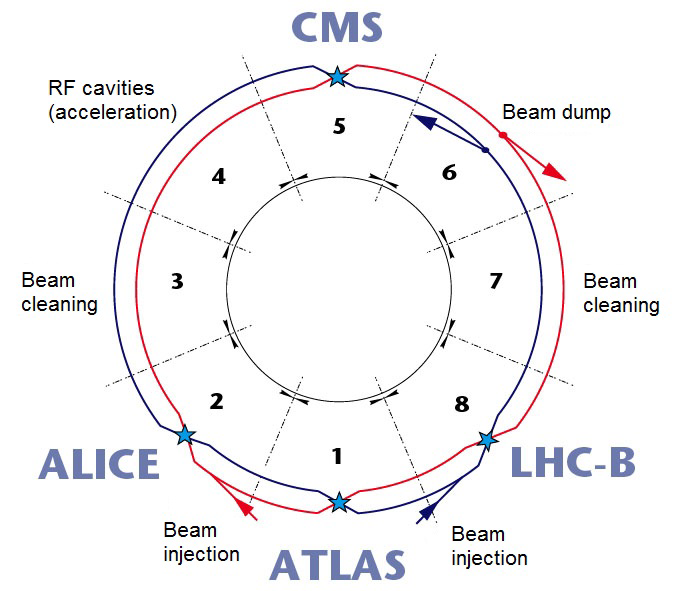
\includegraphics[width=.45\textwidth]{sections/introduction/figures/LHC_accelerator_view.png}};
    \end{tikzpicture}
    \caption{Schematic representation of the LHC~\cite{schematic_representation_lhc}.}
    \label{fig:schematic_representation_lhc}
\end{figure}

In the last operation of the LHC lasting in the period of 2015-2018, called "Run 2", the LHC was accelerating protons to the energy of $E=6.5~\text{TeV}$ in each of its two beams~\cite{cern_main_webpage}. The higher the energy that is attained, the deeper one can study the particle showers obtained during the collisions of the particle beams. They allow for unravelling the fundamentals of particles and interactions between them. There are four collision points in the LHC with different colliders installed that analyse the data from the particle showers: ATLAS\footnote{ATLAS -- A Toroidal LHC ApparatuS.}, CMS\footnote{CMS -- Compact Muon Solenoid.}, ALICE\footnote{ALICE -- A Large Ion Collider Experiment.} and LHCb\footnote{LHCb -- Large Hadron Collider beauty.}. ATLAS and CMS are two large general-purpose detectors whereas ALICE is specialised in heavy-ion physics and LHCb -- in matter-antimatter asymmetry.~\cite[p.~3-21]{evans_marvel_of_technology}

As presented in Fig.~\ref{fig:schematic_representation_lhc}, the LHC is divided into eight sectors. The interaction points, in which the detectors are installed, are situated in four sectors. The~sectors two and eight serve for injecting the initially accelerated beam from other CERN accelerators. In sector four, RF cavities accelerate the~beam at every turn until the particles reach the desired energy. In sector six, the LHC is equipped with a~beam dump system which extracts the~beam from the tunnel in case of a machine failure or if the beam quality deteriorates.~\cite[p.~1-4]{maciejewski_cosimulation_transient_effects_in_magnets}

The LHC is currently being maintained during the so called "Long Shut Down 2" (LS2) for an upgrade of the High-Luminosity LHC which is planned to operate in the~years 2021-2024 referred to as "Run 3". The project aims at increasing the frequency of particle collisions, also described as luminosity. Moreover, the goal of the HL-LHC is to accelerate the particles to the energy of $E=7~\text{TeV}$.~\cite{cern_main_webpage, hl_lhc__main_webpage}